\subsection{Четырехполюсники. Способы формирования описания поведения четырехполюсника. Система параметров}

\begin{center}
	\begin{figure}[h!]
		\center{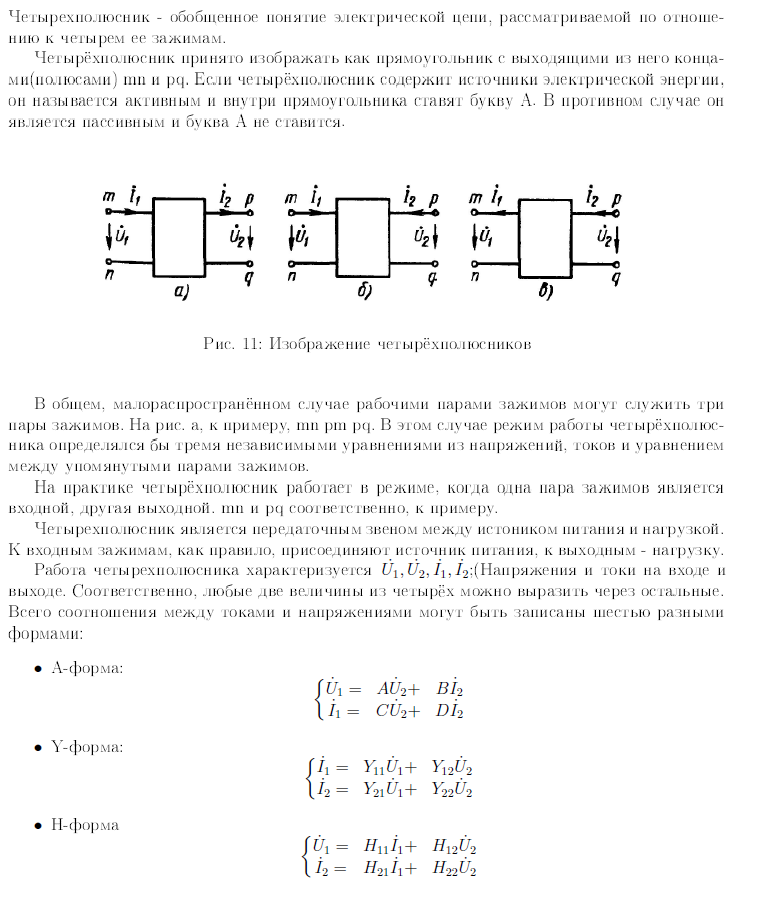
\includegraphics[scale=1]{4p1.png}}
		\caption{}	\end{figure}
\end{center}
\begin{center}
	\begin{figure}[h!]
		\center{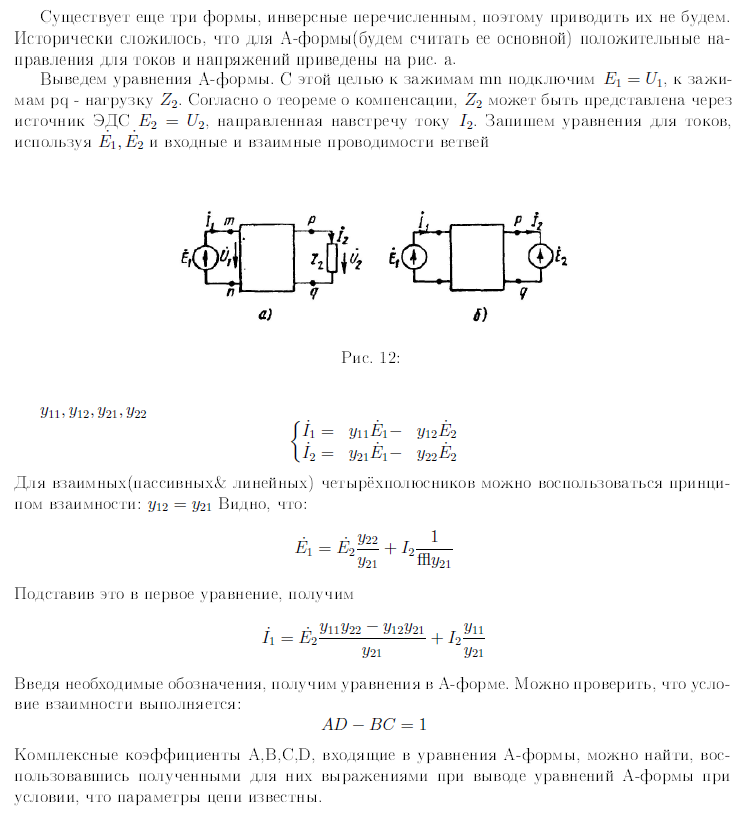
\includegraphics[scale=1]{4p2.png}}
		\caption{}	
	\end{figure}
\end{center}



\pagebreak